\documentclass[../main.tex]{subfiles}
\begin{document}

\chapter{Análise das NR}
 \section{NR-1 - Disposições Gerais}
 Esta é NR que trata das disposições gerais sobre a observância obrigatória das Normas Regulamentadoras (NR) pelas empresas privadas e públicas e pelos órgãos públicos da administração direta e indireta bem como pelos órgãos dos Poderes Legislativo e Judiciário, que possuam empregados regidos pela Consolidação das Leis do Trabalho - CLT.

Segundo ao item 1.2 desta norma:

 \begin{citacao}
 A observância das NR não desobriga as empresas do cumprimento de outras disposições que, com relação à matéria, sejam incluídas em códigos de obras ou regulamentos sanitários dos Estados ou Municípios, e outras, oriundas de convenções e acordos coletivos de trabalho.
 \end{citacao}

 Portanto, para a completa análise do objeto de estudo deste trabalho, recorreremos ao \emph{International Safety Management Code} (\emph{ISM Code}) ou, em português, Código Internacional de Gerenciamento para Operação Segura e para a Prevenção da Poluição, sempre que necessário (ver seção \ref{sec:ISM-code}).

 \section{NR-2 - Inspeção Prévia}
 A NR-2 trata da solicitação de licença prévia para funcionamento instalação antes desta iniciar suas atividades. Esta licença deve ser solicitada junto ao Ministério de Trabalho e Emprego como estipulado nesta mesma NR.

 Considerando que o objeto de estudo deste trabalho não é a empresa em si, mas sim uma embarcação pertencente a esta, torna-se necessário analisar a documentação pertinente para a operação segura da embarcação em suas atividades. Esse documento é o Certificado de Gerenciamento de Segurança exigido pelo Código Internacional de Gerenciamento para Operação Segura e para a Prevenção da Poluição (ISM Code). Esse documento certifica que o sistema de segurança do navio foi submetido a uma auditoria e que ele atende aos requisitos deste código e, ainda, que foi verificado que o Documento de Conformidade da Companhia é aplicável a este tipo de navio.

 Sendo assim, após análise do certificado da companhia, verificou-se que o navio em estudo foi submetido à esta auditoria e atendeu aos requisitos do Código ISM.

 \section{NR-3 - Embargo ou Interdição}
 A NR-3 trata sobre o embargo ou interdição a partir da constatação de situação de trabalho que caracterize risco grave e iminente ao trabalhador. Para esta norma, segundo seu item 3.1.1, essa caracterização é dada por:

 \begin{citacao}
 Considera-se grave e iminente risco toda condição ou situação de trabalho que possa causar acidente ou doença relacionada ao trabalho com lesão grave à integridade física do trabalhador.
 \end{citacao}

 O \emph{ISM Code} não trata exatamente sobre embargo ou interdição de uma atividade, mas diz, em seu capítulo 8, que a empresa deve estabelecer procedimentos para caso acidentes ocorram durante essas atividades.

 Verificou-se que a empresa possui um plano de emergência para este tipo de ocorrência.

 \section{NR-4 - Serviços Especializados em Engenharia de Segurança e em Medicina do Trabalho}
 A NR-4 obriga empresas com empregados sob o regime CLT a manter Serviços Especializados em Engenharia de Segurança e Medicina do Trabalho - SESMT, com a finalidade de promover a saúde e proteger a integridade do trabalhador no local de trabalho.
 
 O dimensionamento do SESMT vincula-se à gradação do risco da atividade principal e ao número total de empregados do estabelecimento, constantes, respectivamente, dos Quadros I e II, anexos, dessa NR.
 
 Embora o objeto em análise neste trabalho seja uma embarcação, segundo o item 4.2.1 da NR-4, para fins de dimensionamento do SESMT, a embarcação, por possuir menos de 1 (um) mil empregados, deve ser considerada integrante da empresa responsável. Portanto, o dimensionamento deverá então ser realizado para toda a empresa e não somente para a embarcação.  
 
 Quanto à gradação do risco da atividade, a empresa se enquadra no código de Classificação Nacional de Atividades Econômicas (CNAE) \textbf{50.30-1 - Navegação de Apoio} e, por conseguinte, possui grau de risco 4 conforme Quadro I da NR-4.
 
 Quanto ao número total de empregados, a empresa conta com 405 empregados próprios, sendo que, deste total, xx trabalham na embarcação.% e xx empregados de empresas terceirizadas.
 
 Como já discutido, estas duas informações, grau de risco e número de funcionários, permite dimensionar o SESMT da empresa conforme estipulado pelo Quadro II, anexo na NR-4, mostrado na \autoref{fig:board-II_NR-4}.
 
 \begin{figure}[H]
  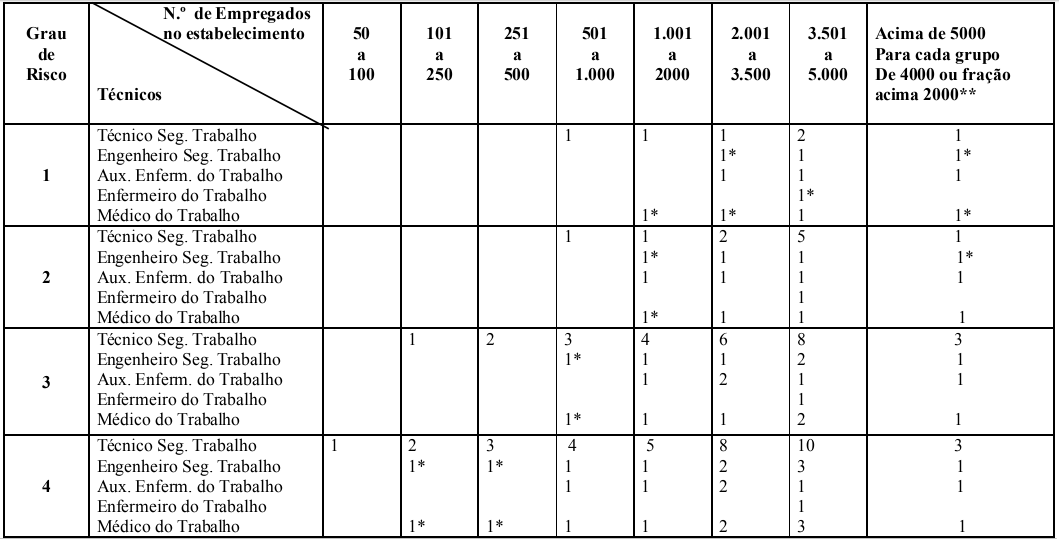
\includegraphics[scale=0.4]{quadroII_SESMT}  
  \caption{Quadro II - Anexo NR-4}  
  \label{fig:board-II_NR-4}
 \end{figure}
 
 Verificou-se o atendimento à essa NR, considerando que a empresa possui em seu quadro composição do SESMT um Engenheiro de Segurança do Trabalho e três Técnicos de Segurança do Trabalho, todos com formação e registro profissional em conformidade com o disposto na regulamentação da profissão e nos instrumentos normativos emitidos pelo respectivo Conselho Profissional. % CREA - Engenheiro de Seg, MTE - Técnicos
 
 À respeito das competências dos Serviços Especializados em Engenharia de Segurança e em Medicina do Trabalho, a empresa cumpre com todas as alíneas do item 4.12 e mantém:
 % exemplo 1
 % exemplo 2
 
 \section{NR-5 - Comissão Interna de Prevenção de Acidentes}
 A Comissão Interna de Prevenção de Acidentes - CIPA - tem como objetivo a prevenção de acidentes e doenças decorrentes do trabalho, de modo a tornar compatível permanentemente o trabalho com a preservação da vida e a promoção da saúde do trabalhador.
 
 
\end{document}